% Generated from frozen structural results. Requires booktabs and graphicx.
\begin{table*}[t]
\centering\small
\caption{Exact structural gaps. Each cell is base / holdout; cohorts contain 1323 / 2115 shapes. $\Delta=U-\mathrm{OPT}$ is an integer record count and $r=\Delta/\mathrm{OPT}$. Every shape has equal weight.}
\label{tab:structural-exact-gaps}
\begin{tabular}{lrrrr}
\toprule
Method & OPT hits & Mean $\Delta$ & Max $\Delta$ & Max $r$ (\%)\\
\midrule
First-fit & 96 / 20 & 2.054 / 3.022 & 6 / 8 & 100.0 / 140.0\\
AB & 1123 / 1780 & 0.151 / 0.158 & 1 / 1 & 25.0 / 20.0\\
AB + pair & 1125 / 1796 & 0.150 / 0.151 & 1 / 1 & 25.0 / 20.0\\
AB + 3 & 1314 / 2073 & 0.007 / 0.020 & 1 / 1 & 25.0 / 20.0\\
AB + 3$\to$4 & 1321 / 2112 & 0.002 / 0.001 & 1 / 1 & 25.0 / 20.0\\
Exact OPT & 1323 / 2115 & 0.000 / 0.000 & 0 / 0 & 0.0 / 0.0\\
\bottomrule\end{tabular}\end{table*}
First-fit uses the smallest available ancestor color and is depth coloring on these skeletons. Both cohorts use the same algorithms and independently checked canonical skeletons and record-parent forests. These results measure structural optimality gaps; they are not PIR timings.
The final five failures are S0606, S0710, H1199, H1265, and H1285. Each has $U-\mathrm{OPT}=1$; their exact relative gaps are $1/4$, $1/4$, $1/5$, $1/5$, and $1/6$, respectively. This finite observation does not imply a constant additive approximation guarantee.
\begin{figure*}[t]\centering
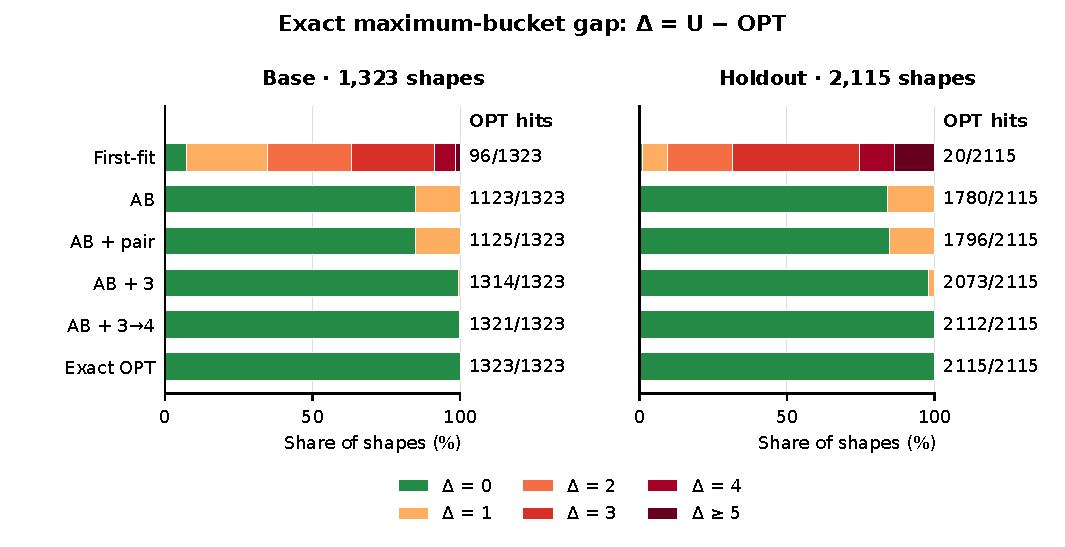
\includegraphics[width=\textwidth]{figures/absolute_gap_distribution_compact.pdf}
\caption{Exact integer gap distribution on the two frozen censuses; gaps of five or more are grouped. Green denotes an attained optimum; labels give exact hit counts. The final five positive gaps are all one record, but the worst relative gaps remain 25\% and 20\%. These are structural counts, not PIR costs or deployment success rates.}
\label{fig:structural-gap-distribution}\end{figure*}
